\let\negmedspace\undefined
\let\negthickspace\undefined
\documentclass[journal]{IEEEtran}
\usepackage[a5paper, margin=10mm, onecolumn]{geometry}
%\usepackage{lmodern} % Ensure lmodern is loaded for pdflatex
\usepackage{tfrupee} % Include tfrupee package

\setlength{\headheight}{1cm} % Set the height of the header box
\setlength{\headsep}{0mm}     % Set the distance between the header box and the top of the text

\usepackage{gvv-book}
\usepackage{gvv}
\usepackage{cite}
\usepackage{amsmath,amssymb,amsfonts,amsthm}
\usepackage{algorithmic}
\usepackage{graphicx}
\usepackage{textcomp}
\usepackage{xcolor}
\usepackage{txfonts}
\usepackage{listings}
\usepackage{enumitem}
\usepackage{mathtools}
\usepackage{gensymb}
\usepackage{comment}
\usepackage[breaklinks=true]{hyperref}
\usepackage{tkz-euclide} 
\usepackage{listings}
% \usepackage{gvv}                                        
\def\inputGnumericTable{}                                 
\usepackage[latin1]{inputenc}                                
\usepackage{color}                                            
\usepackage{array}                                            
\usepackage{longtable}                                       
\usepackage{calc}                                             
\usepackage{multirow}                                         
\usepackage{hhline}                                           
\usepackage{ifthen}                                           
\usepackage{lscape}
\begin{document}

\bibliographystyle{IEEEtran}
\vspace{3cm}

\title{1.8.23}
\author{EE24BTECH11012 - Bhavanisankar G S}
% \maketitle
% \newpage
% \bigskip
{\let\newpage\relax\maketitle}

\renewcommand{\thefigure}{\theenumi}
\renewcommand{\thetable}{\theenumi}
\setlength{\intextsep}{10pt} % Space between text and floats


\numberwithin{equation}{enumi}
\numberwithin{figure}{enumi}
\renewcommand{\thetable}{\theenumi}

\textbf{QUESTION}:\\
If \myvec{\emph{a},\emph{b}} is the mid-point of the line segment joining the points \vec{A} \myvec{10,-6} and \vec{B} \myvec{\emph{k}, 4} and $ \emph{a} - 2\emph{b} = 18 $, find the value of \emph{a}, \emph{b} and the distance \vec{AB} . \\
\textbf{SOLUTION}: \\
\begin{tabular}[12pt]{|c|c|c|}
    \hline
    \textbf{Variable name} & \textbf{Description} & \textbf{Formula}\\ 
    \hline
		$A$ & $\myvec{2 \\ 3 \\ -4}$ &  \\
    \hline 
		$B$ & $\myvec{3 \\ -4 \\ -5}$ & \\
    \hline
		$C$ & $\myvec{3 \\ 2 \\ -3}$ &   \\
    \hline   
	$D$ & Distance of the point from the origin. &  $\abs{\vec{D}\myvec{a\\b\\c}}=\sqrt{a^2+b^2+c^2}$ = ? (\since \abs{D} is the distance of the point D from the origin . \\
	\hline
\end{tabular}

 \\ \\ \\
We know that if $\vec{M}$ is the mid-point of $\vec{AB}$, then \\
	 $$ \vec{M} = \frac{\vec{A} + \vec{B}}{2} \\ $$
	$$ \myvec{ \emph{a} \\ \emph{b} } = \frac{\myvec{ 10 \\ -6 } + \myvec{ \emph{k} \\ 4 }}{2} \\ $$
	 $$\implies \boxed{ \textbf{\emph{b} = -1}} \\ $$
	 $$\emph{a} = 18 + 2\emph{b} \\$$
	 $$\implies \boxed{ \textbf{\emph{a} = 16}} \\$$
	 $$\emph{k} = 2\emph{a} - 10 \\ $$
	 $$\implies \boxed {\textbf{\emph{k} = 22}} \\$$
	$$\norm {\vec{B-A}} = \sqrt{\myvec{B-A}^T\myvec{B-A}} \\$$
	                $$   = \sqrt{\myvec{12 & 10}\myvec{12 \\ 10}} \\$$ 
			 $$\textbf {\boxed {\norm{\vec{AB}}  = 2\sqrt{61}}} $ \\$$

			 \begin{figure}[h]
				 \centering
				 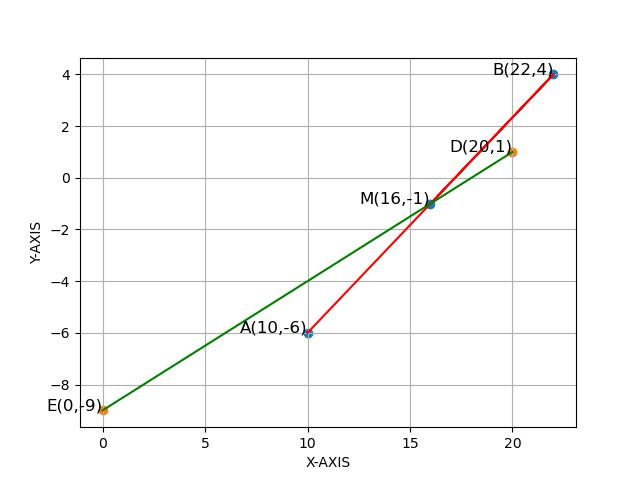
\includegraphics[width=0.8\textwidth]{figs/value.jpg}
				 \caption{A plot of the given question.}
				 \label{fig:Plot1}
			 \end{figure}


\end{document}
